  \documentclass{journal}[IEEEtran, twocolumn]             % No modificar

% PASO 1. Reemplace "Práctica 1" por el número de la práctica que corresponda
\newcommand{\dochead}{Practice N°2}     

% PASO 2. Verifique el título de la práctica corresponda.
\newcommand{\docsubhead}{PSD and Random Signals}  

% PASO 3. Reemplace "B1A - 02" por el grupo de la asignatura y el número de su grupo de laboratorio
\newcommand{\teamname}{B2}     

% PASO 4. OPCIONAL: Reemplace "\docsubhead \docsubhead" por el título del documento en caso de requerirse.
\newcommand{\titulo}{\dochead: \docsubhead}      

% PASO 5. Reemplace "31 de diciembre de 2030" por la fecha de su documento
\newcommand{\fecha}{March 10, 2024}      

% To load packages
\usepackage{microtype}
\usepackage[T1]{fontenc}
\usepackage[utf8]{inputenc} 
\usepackage[english]{babel}
\usepackage[letterpaper,left=2.0cm,top=2.0cm,right=2.0cm,bottom=4.0cm]{geometry}
\usepackage{amsmath}
\usepackage{amsfonts}
\usepackage{fancyhdr}
\usepackage{fancyvrb}
\usepackage{listings}
\usepackage{array}
\usepackage{graphicx,color,enumerate}	
\usepackage{multirow} 
\usepackage{multicol}
\usepackage{authblk}
\usepackage{charter}    
\usepackage{titling}
\usepackage{url}
\usepackage{hyperref}
\usepackage{xcolor}
\usepackage{tabularx}
\usepackage{tikz}
\usepackage{float}
\usepackage{booktabs}
\usepackage{longtable}
\usepackage{adjustbox}
\usepackage{subcaption}
\usepackage{colortbl}
\usepackage{tcolorbox}

\definecolor{uisgreen}{RGB}{125,194,3}
\definecolor{gray97}{gray}{.97}
\definecolor{gray75}{gray}{.75}
\definecolor{gray45}{gray}{.45}

\setlength{\droptitle}{-1.8cm}
\pagestyle{fancy}

%%% Header definition
\headheight=60pt 						% header height 
\renewcommand{\headrulewidth}{4pt}
\let\oldheadrule\headrule% Copy \headrule into \oldheadrule
\renewcommand{\headrule}{\color{uisgreen}\oldheadrule}

\fancyhead[L]							% left header 
{	\begin{minipage}{2.5cm}
		
\includegraphics[scale=0.3]{./figs/uislogohoriz.png} 
	\end{minipage}	
	\begin{minipage}{5cm}
	    \color{uisgreen}
	    \footnotesize {\textsf{Universidad Industrial de Santander\\ 
				Escuela de Ingenierías Eléctrica, \\
				Electrónica y de Telecomunicaciones	}}	
	\end{minipage}
}
\fancyhead[R] { 							%la "C" indica al centro
	\begin{minipage}{8cm}
	    \color{uisgreen}
	    \begin{flushright}
    	    \small{\textsf{Communications II - LAB (27145)}} \\
            \normalsize{\textsf{\dochead: \textbf{\docsubhead}}} \\
    	    \small{\textsf{Group: \textbf{\teamname}}}
	    \end{flushright}
    \end{minipage}
    \begin{minipage}{1.2cm}
		
\includegraphics[width=1.0\textwidth]{./figs/logoE3T.png} 
	\end{minipage}	
}
%%% End header definition

\lstset{ frame=Ltb,
     framerule=0pt,
     aboveskip=5pt,
     framextopmargin=3pt,
     framexbottommargin=3pt,
     framexleftmargin=0.4cm,
     framesep=0pt,
     rulesep=.4pt,
     backgroundcolor=\color{gray97},
     rulesepcolor=\color{black},
     %
     stringstyle=\ttfamily\color{red!50!brown},
     showstringspaces = false,
     basicstyle=\small\ttfamily,
     commentstyle=\color{gray45},
     keywordstyle=\color{blue}\bfseries,
     %
     numbers=left,
     numbersep=5pt,
     numberstyle=\tiny,
     numberfirstline = false,
     breaklines=true,
   }

% minimizar fragmentado de listados
\lstnewenvironment{listing}[1][]
   {\lstset{#1}\pagebreak[0]}{\pagebreak[0]}

\lstdefinestyle{consola}
   {basicstyle=\scriptsize\bf\ttfamily,
    backgroundcolor=\color{gray75},
   }

\lstdefinestyle{C}
   {language=C,
   }

             % No modificar


\begin{document}                    % No modificar

\title{\textbf{\titulo}}            % No modificar

% PASO 6. Agregar aquí el nombre y código de los autores.  
\author{
Jeanpaull Valencia Quintero - 2200496 \\
Ramon Stiven Sarmiento Castro - 2200503 \\
Juan Manuel Tellez Calderon - 2194235
}

\affil{\small{Escuela de Ingenierías Eléctrica, Electrónica y de Telecomunicaciones} \\ % No modificar
\small{Universidad Industrial de Santander}} % No modificar

\date{\fecha}                       % No modificar

\maketitle                          % No modificar
\thispagestyle{fancy}               % No modificar

%---------------------------------------------------------------
% PASO 7. **..**...****INICIE SU DOCUMENTO DESDE AQUI***...**...
%%%%% A PARTIR DE AQUÍ EDITE EL DOCUMENTO PARA AGREGAR TODO EL CONTENIDO REQUERIDO PARA EL ENTREGABLE CORRESPONDIENTE
%%%%  Todo el contenido a partir de este punto es SOLAMENTE ILUSTRATIVO.

\color{black}

\begin{multicols}{2}

\begin{abstract}
In this laboratory practice, an exhaustive analysis of the inherent properties of various types of signals is carried out, ranging from random signals to more complex and structured signals such as image and audio signals. The primary purpose of this practice is to unravel and thoroughly understand the interaction and correspondence that these signals maintain with different types of modulations and with the Power Spectral Density (PSD). PSD is defined as a measure of how the power of a signal is distributed across the frequency spectrum.

\end{abstract}

\section{Methodology}

The methodology for this practice was divided into the next four components:

\subsection{Analysis and use of the flowchart for random binary signals}

For the configuration of the Random Binary Signals flowchart, all content was downloaded based on the repository provided by the practice file. Since the content was already constructed, the random bipolar characterization was undertaken. Figure \ref{fig:figA} depicted this structure. The flowchart had a relevant parameter: SPS (Samples per second). Therefore, the following values were varied:

\begin{figure}[H]
        \centering
            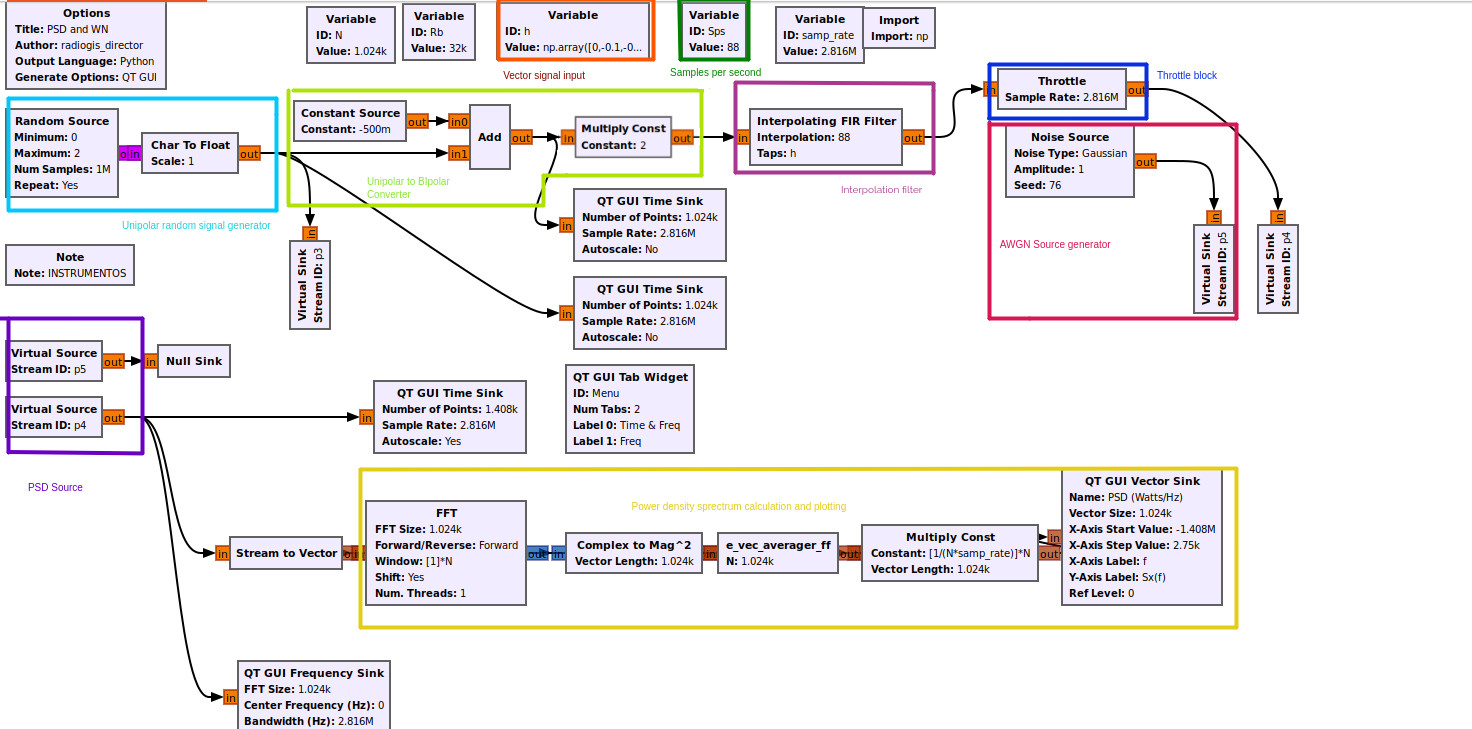
\includegraphics[width=0.65\columnwidth]{figs/Structure.jpg}
        \caption{\centering Structure of the Random Bipolar and PSD plotter}
        \label{fig:figA}
\end{figure}

Subsequently, the use of this image was made to describe the functioning of the individual blocks and the system.\\
\\
SPS = [1,4,8,16]

\subsection{Application of AWGN}

AWGN was applied by changing sources in the flowchart, the Gaussian Noise section could be observed in Figure \ref{fig:figA}; it only required changing the source of the PSD plotter to obtain the PSD of the Gaussian noise and analyze it.

\subsection{Use of real images or signals}

For the analysis of real signals, both an image and an audio signal were used. The switch to File Source and Unpack K Bits was executed. Figure \ref{fig:figB} served as evidence of this change, with the aim of obtaining suitable results in the analysis of both signal types.

\begin{figure}[H]
    \centering
        \centering
        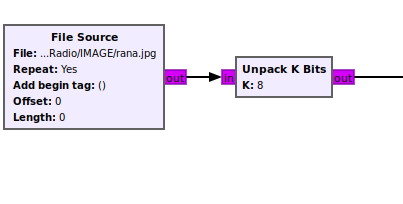
\includegraphics[width=0.35\columnwidth]{figs/Signal.png}
    \caption{Switching from random source to file source.}
    \label{fig:figB}
\end{figure}


\subsection{Applications and control questions}

From all these configurations, the various signals requested were generated, thereby addressing the questions posed in the guide.
    
\section{Results and analysis}

As with the methodology, the analysis of results was based on the previously defined structure; from that moment on, a synchronized effort was carried out, which constituted the majority of the work.

\subsection{Analysis of the Bipolar random signal generator parameters}

Using the defined structure, in Figure \ref{fig:figA}, the modification of the samples per second parameter was carried out, from which it was observed that increasing the samples per second allowed for a better constituted signal. But how could this have been possible? What did the quantity of samples have to do with it? It turned out that, as could be compared in Figure \ref{fig:FigC}.

\begin{figure}[H]
    \centering
        \centering
        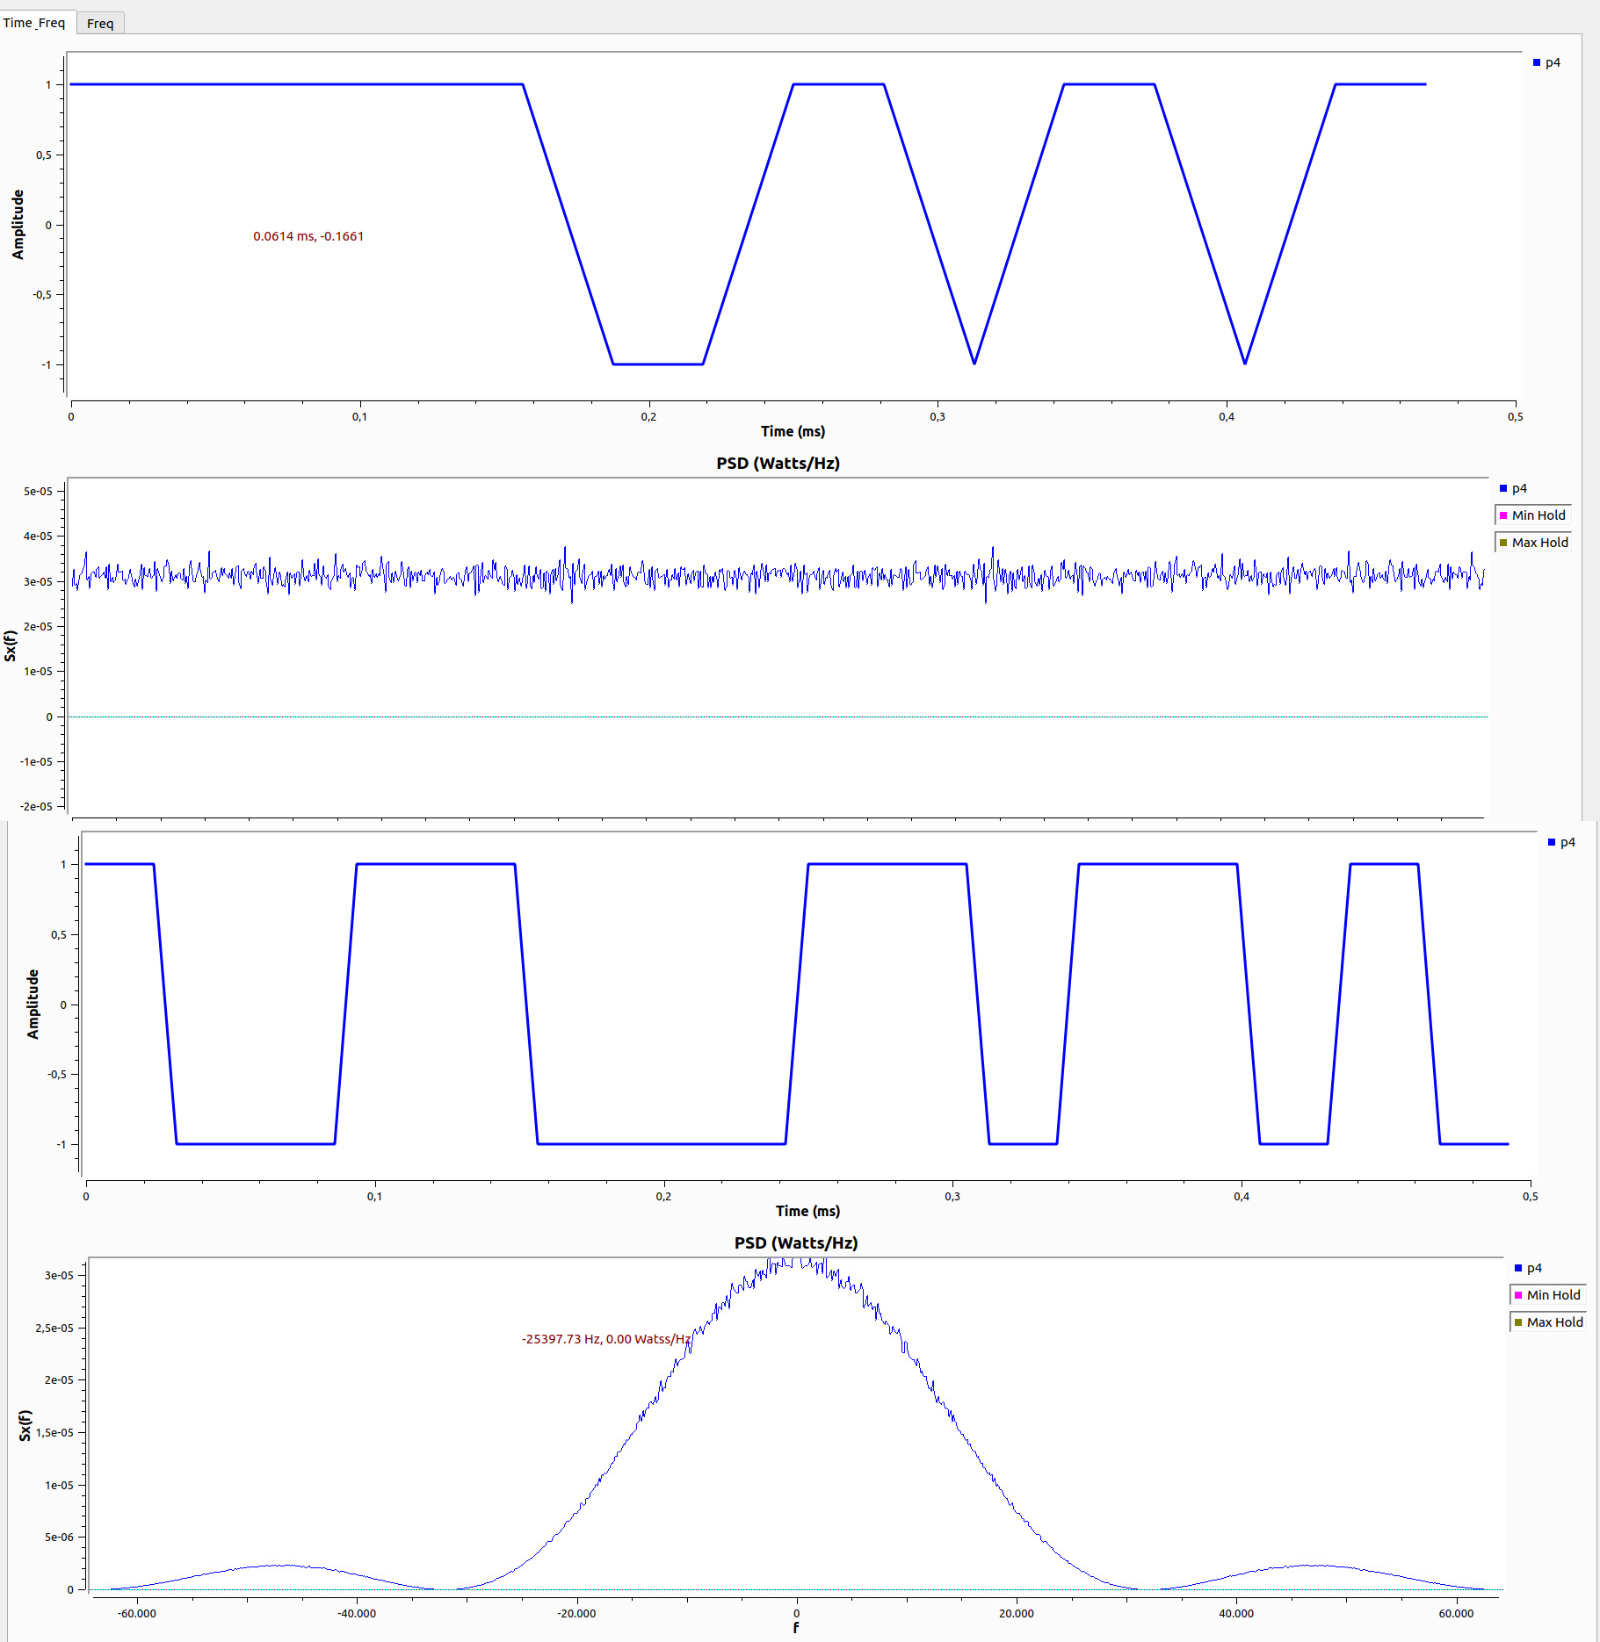
\includegraphics[width=0.5\columnwidth]{figs/SP16.png}
    \caption{Comparison between SPS = 1 and SPS = 6.}
    \label{fig:FigC}
\end{figure}

the interpolation filter took the stream signals and added the quantity of samples in the interpolation, thus utilizing the most useful parts of the random signals. In fact, that was why in real-time, the signal started to take on a square structure, as the random signal was expanded to achieve such compatibility.

The following table summarized the results of changing the samples per second:

\begin{table}[H]
    \begin{tabular}{ |p{0.5cm}|p{1.1cm}|p{1.9cm}|p{1.1cm}|p{1.5cm}| }
    \hline
    \rowcolor{green!30}
    Sps & Band width (Hz) & Bit time (sec) & Bit rate (Bps) & Sample freq (Hz)\\
    \hline
    16 & 32000 & 0,00003125 & 32000 & 512000 \\
    8 & 32000 & 0,00003125 & 32000 & 256000 \\
    4 & 32000 & 0,00003125 & 32000 & 128000\\
    \hline
    \rowcolor{green!30}
    1 & 32000 & 0,00003125 & 32000 & 32000 \\
    \hline

    \hline
    \end{tabular}
    \caption{Change of Sps parameter}
    \label{tab:tabA}
    \end{table}

Some observations from Table \ref{tab:tabA} were focused on maintaining bandwidth, which made sense as it defined the minimum channel for information transmission, usually determined by the bit rate. Only the sampling frequency changed, depending on the number of samples, thus increasing due to interpolation.

\subsection{WGN insertion analysis}
For the analysis of Gaussian noise, the sources or virtual sources shown in Figure \ref{fig:figA} were replaced. With these changes, the PSD plotter now observed a Gaussian white noise source. Figure \ref{fig:figE} served as evidence of this behavior.

\begin{figure}[H]
    \centering
        \centering
        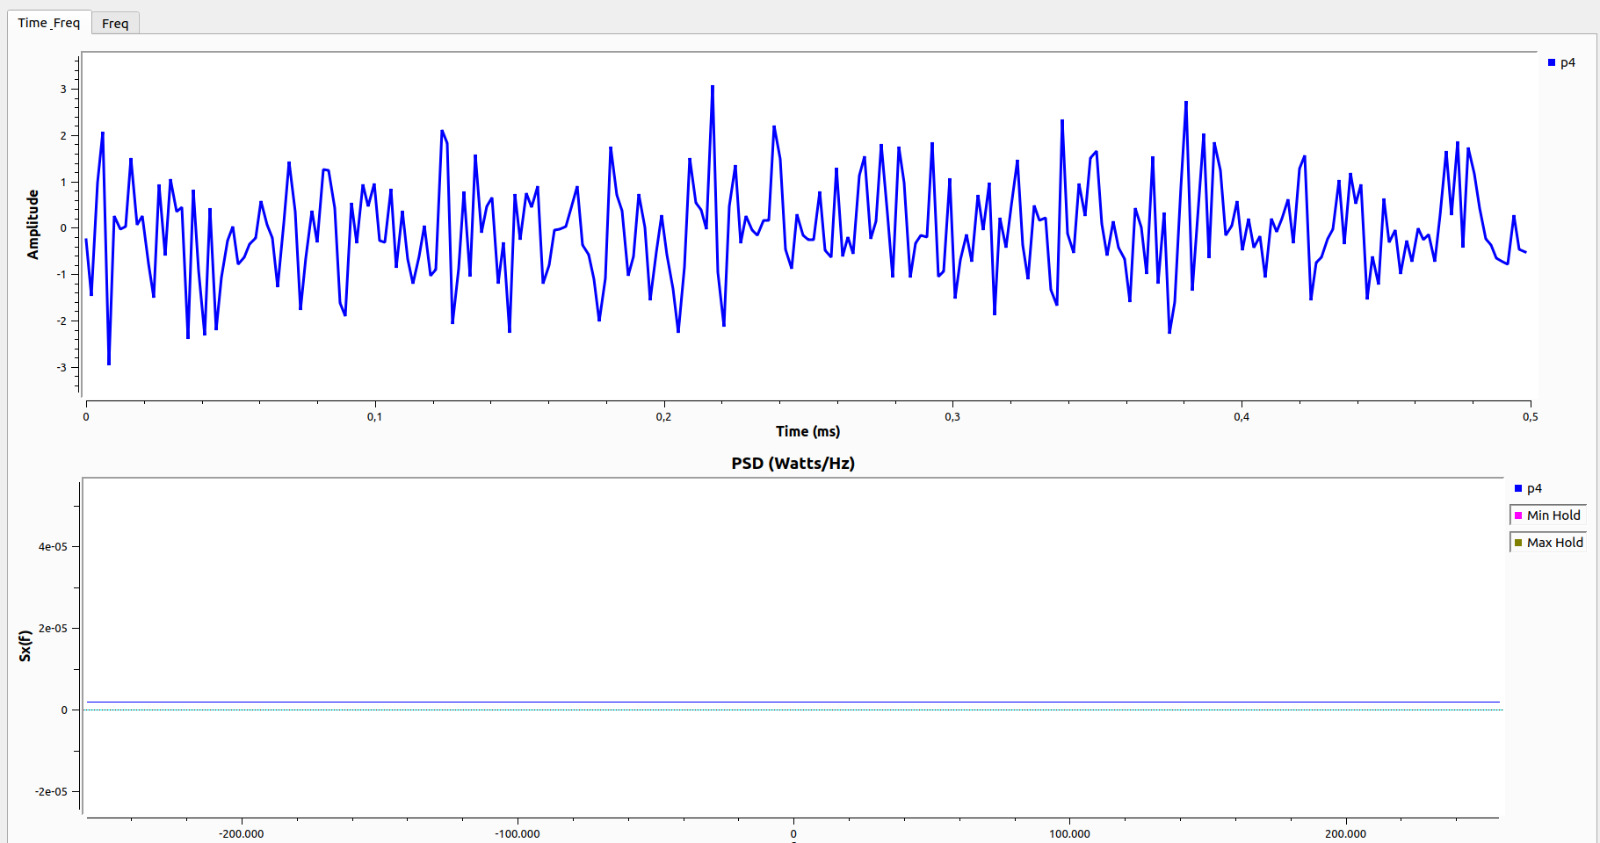
\includegraphics[width=0.7\columnwidth]{figs/AWGN.png}
    \caption{Switching from random source to file source}
    \label{fig:figE}
\end{figure}

One of the first observations we made is that Gaussian noise possesses somewhat unique properties, such as its bandwidth. Gaussian noise doesn't inherently carry any information nor does it have an associated sampling frequency; ideally, its bandwidth would be infinite unless limited by the channel through which it travels.

\subsection{Image and sound source analysis}

For that analysis, the random unipolar signal source from Figure \ref{fig:figB} was replaced with the file source from Figure \ref{fig:figB}, facilitating the use of the proposed audio file and image. Following this exchange, the PSD of these files was observed. Figure \ref{fig:figF} illustrated the PSD of an image.

\begin{figure}[H]
    \centering
        \centering
        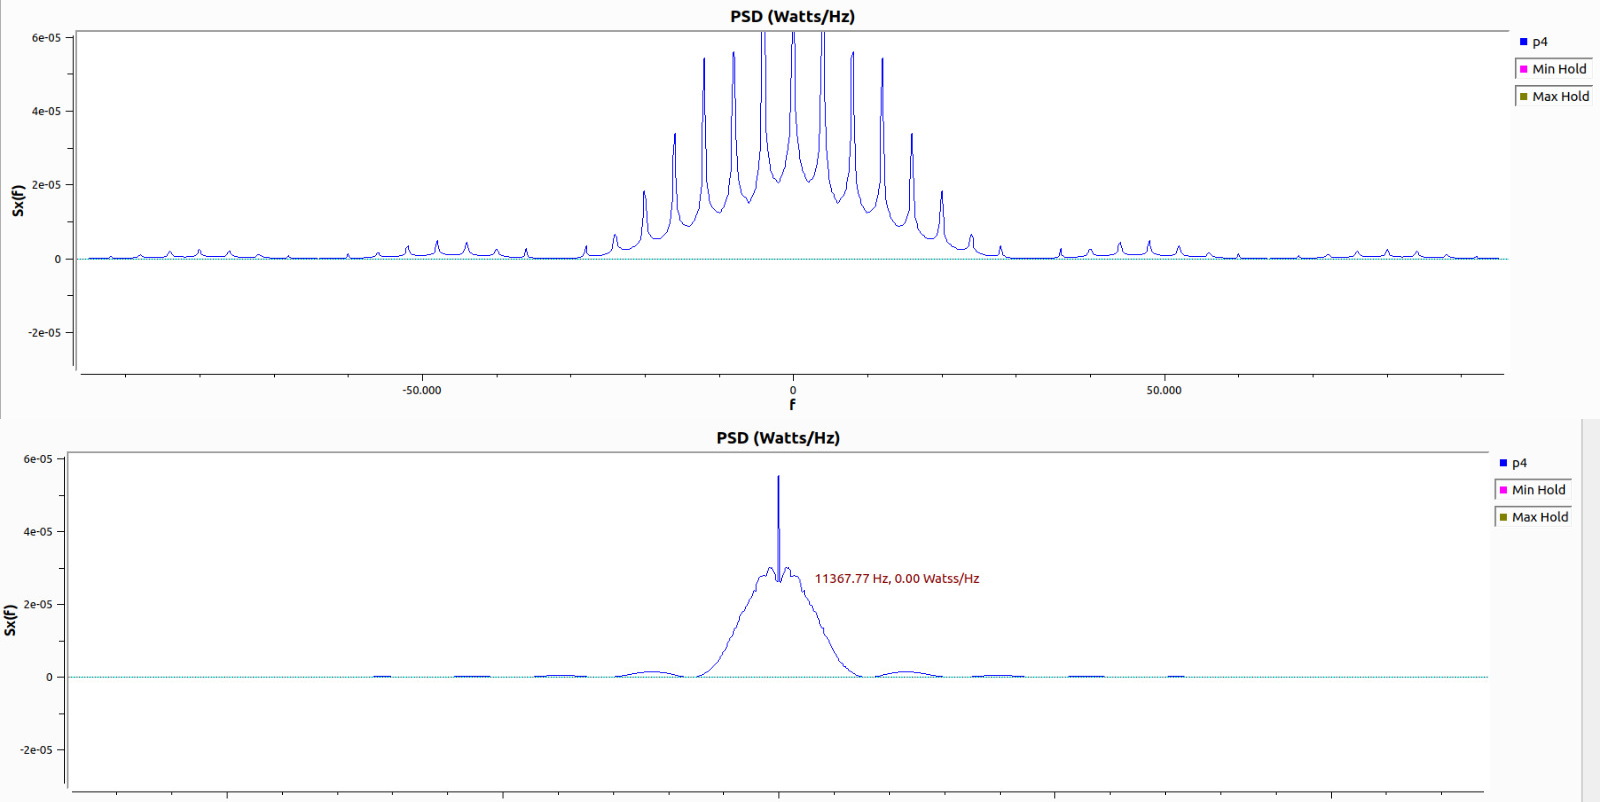
\includegraphics[width=0.65\columnwidth]{figs/im_aud.png}
    \caption{Image and Audio PSD}
    \label{fig:figF}
\end{figure}

Notably, the image exhibited distinctive properties. Initially, a peak at the central frequency became apparent. This phenomenon was typically ascribed to the grouping of pixels or color information in nearby regions, particularly due to their average values.

Figure \ref{fig:figF}, also shows the PSD of the audio file.
In this case, the audio manifested a greater abundance of harmonics in its power spectral density. This was primarily a consequence of employing various instruments over time, contributing to the overall PSD.

\subsection{Control questions analysis}

Prior to the section, reference was made to a compilation of images representing all the modifications made during the practice. This collage was presented in Figure \ref{fig:figTRANS}.

\begin{figure}[H]
    \centering
        \centering
        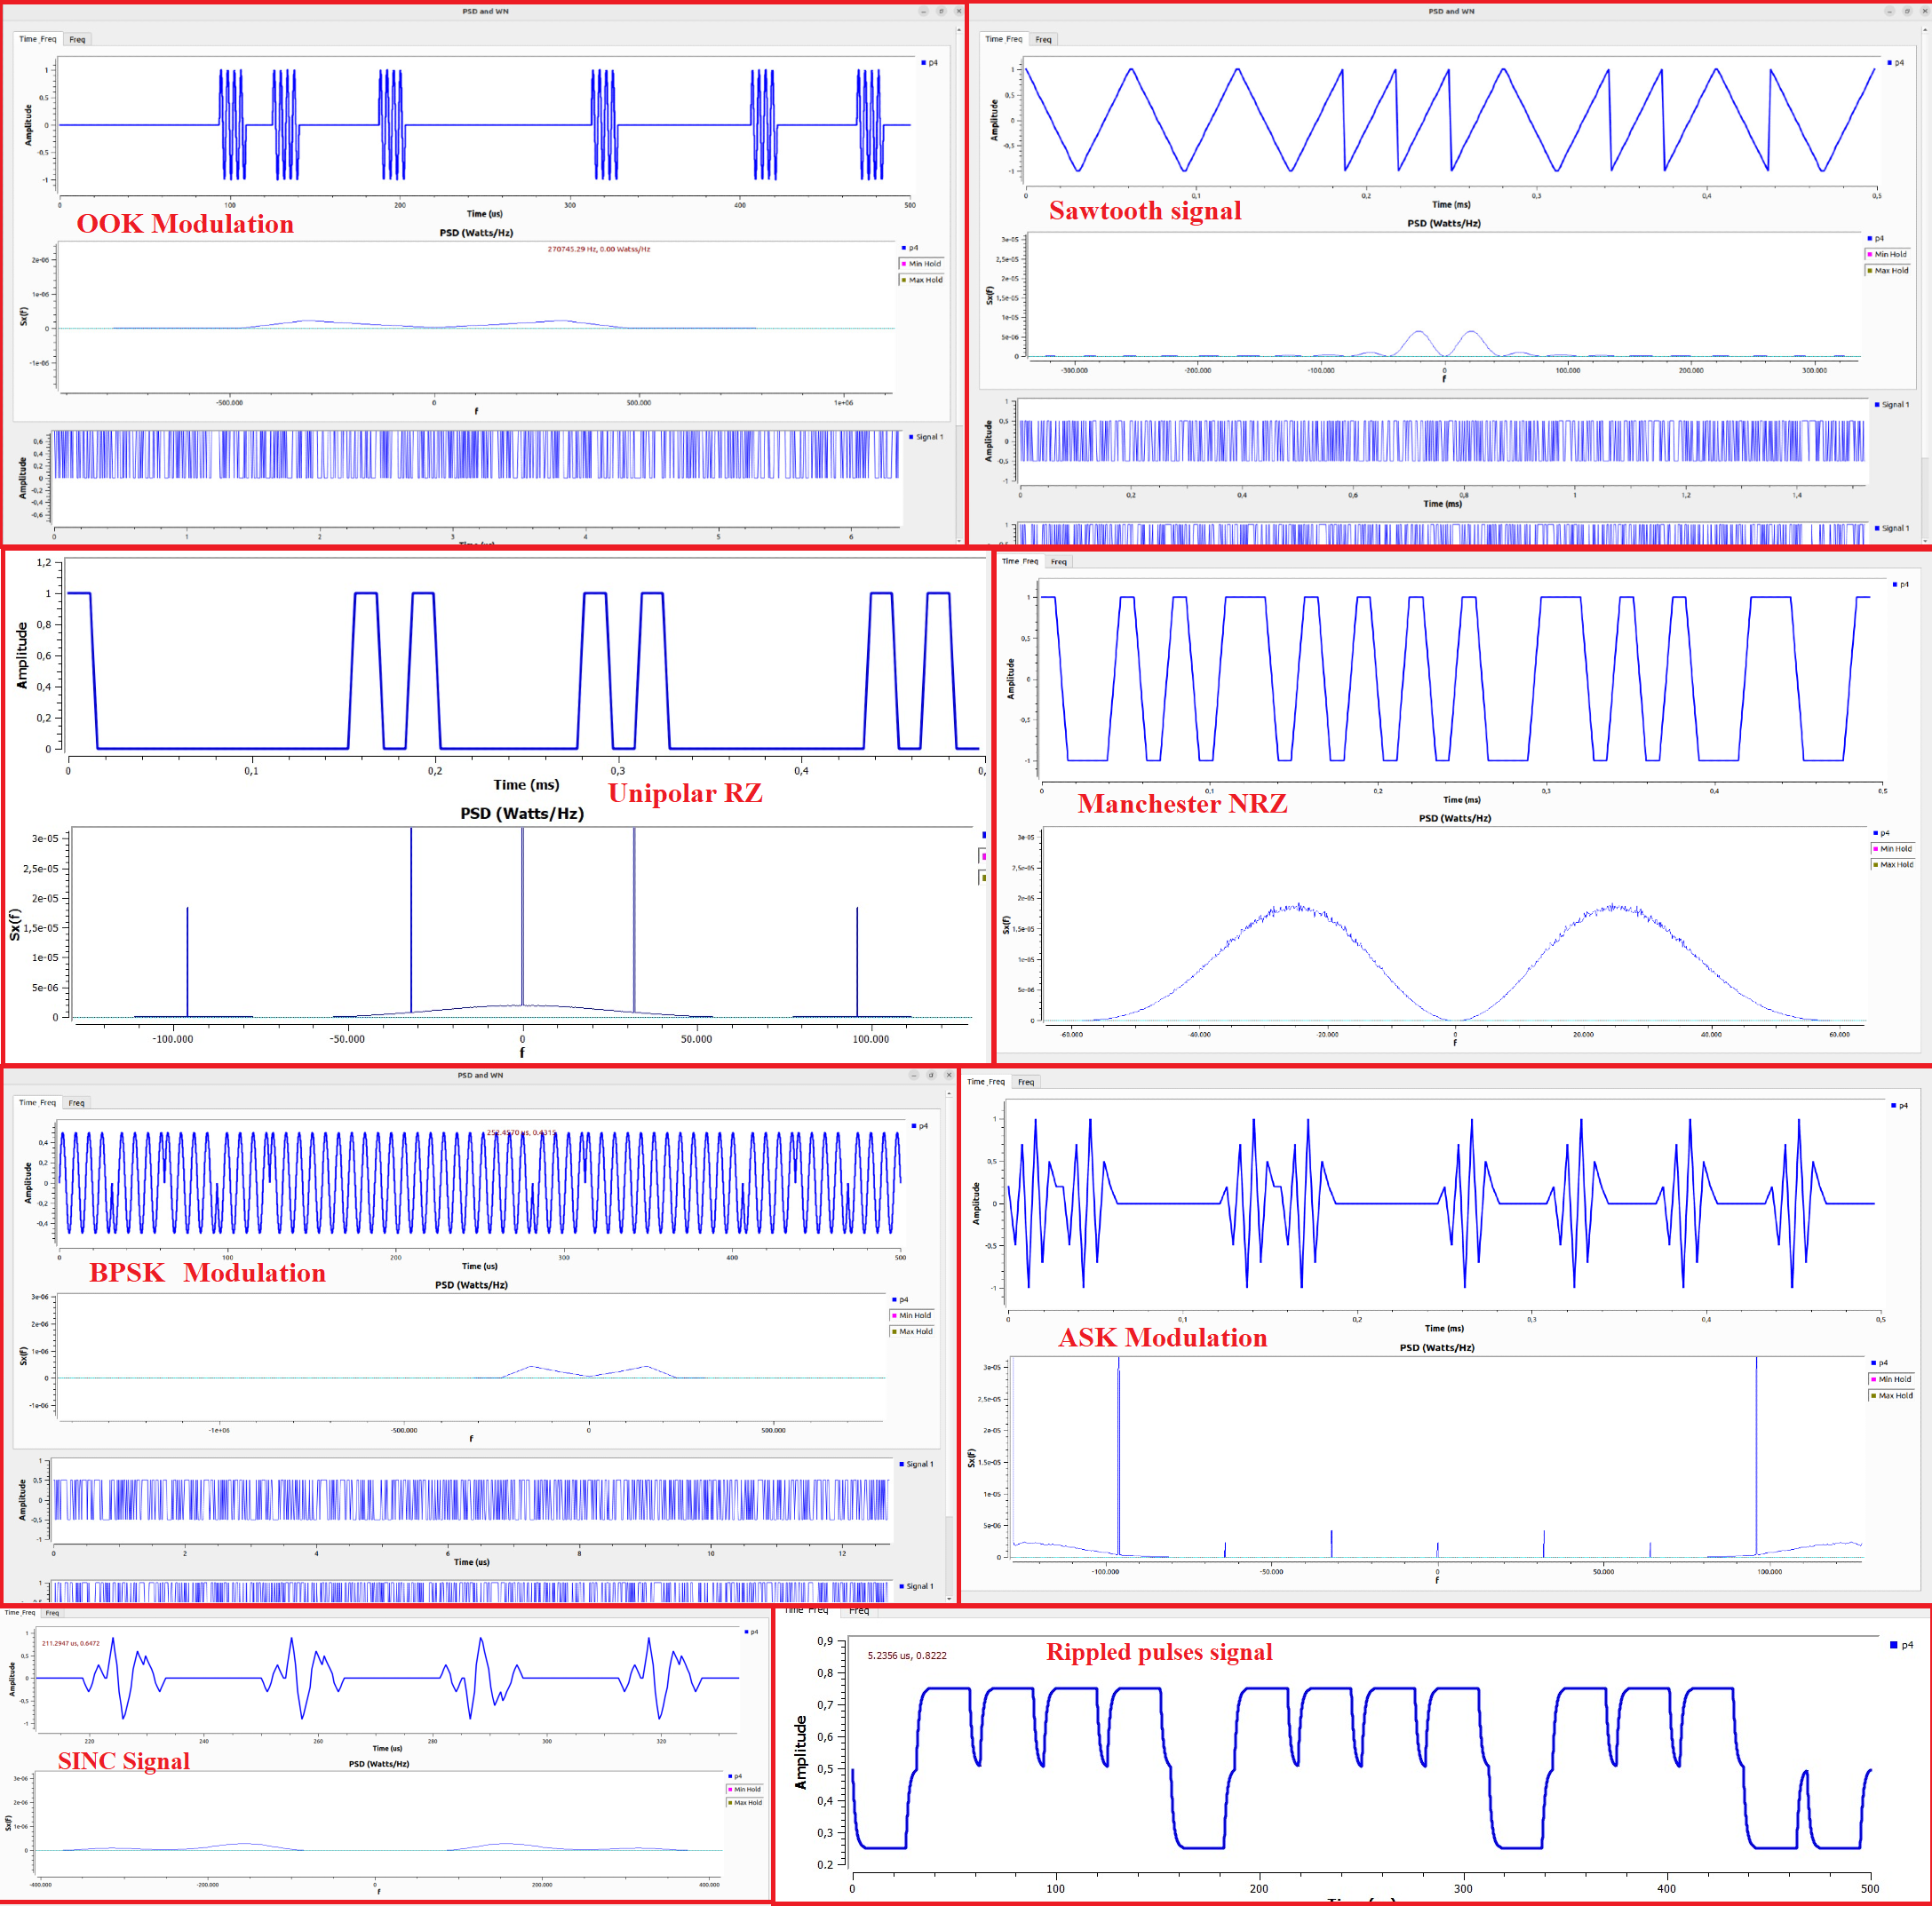
\includegraphics[width=0.7\columnwidth]{figs/Transfor.png}
    \caption{Output signals obtained by modifying the h parameter}
    \label{fig:figTRANS}
\end{figure}

\renewcommand{\labelenumi}{{\Alph{enumi}})}
\begin{enumerate}
    \item The block system highlighted in green in Figure \ref{fig:figA} converted the signal into bipolar to maintain an average of 0, thereby improving the visibility of the fundamental harmonic in the Power Spectral Density (PSD). In contrast, unipolar signals had a more pronounced fundamental harmonic. This block reduced the signal by 0.5 units and then multiplied it by 2 to place it in a final range of [-1, 1].

    \item \textbf{1.} In the interpolation block, the \textit{SPS} value exists because it determines the number of samples to be added in the interpolation; moreover, this parameter was determined from the length of the variable h, which is the interpolation vector.\\
    \\
    \textbf{2.} In GNURadio, the combination of \textit{Virtual Sink} and \textit{Virtual Source} blocks was used to analyze the different signals, which were connected by means of an ID parameter, so, to analyze p3, its respective ID was placed in the Virtual Source block.\\
    \\
    \textbf{3.} The bandwidth remained the same, because although the samples were increased, the sampling rate in the Throttle block was also increased by the same amount. $\frac{1}{T_b}$\\
    \\
    \textbf{4.} From the previous item, it can be deduced that the bandwidth of the signal \textit{p3}, the one before the interpolation block, is the same as defined by the variable \textit{Rb}.\\

    \item The difference in the PSD of an image and an audio signal is based on the way in which the information is distributed, an audio signal can have more variations in its intensity over time, on the other hand an image also has variations in its intensity but with the difference that it can have constant information because the colors of the image can remain the same.

    \item the throttle block would copy input elements to the output, consuming input samples at an average rate. It is primarily included for hardware devices without a defined rate (real-time), but in this case it regulated the sampling rate to be perceptible to humans.

    \item To analyze the unipolar NRZ signal, the offset value was changed in the flowchart, making it zero, and the multiplication constant was set to one, thus, as shown in figure \ref{fig:unipolar_PSD}, the signal already has a DC power component, which was not the case with the bipolar NRZ.\begin{figure}[H]
    \centering
        \centering
        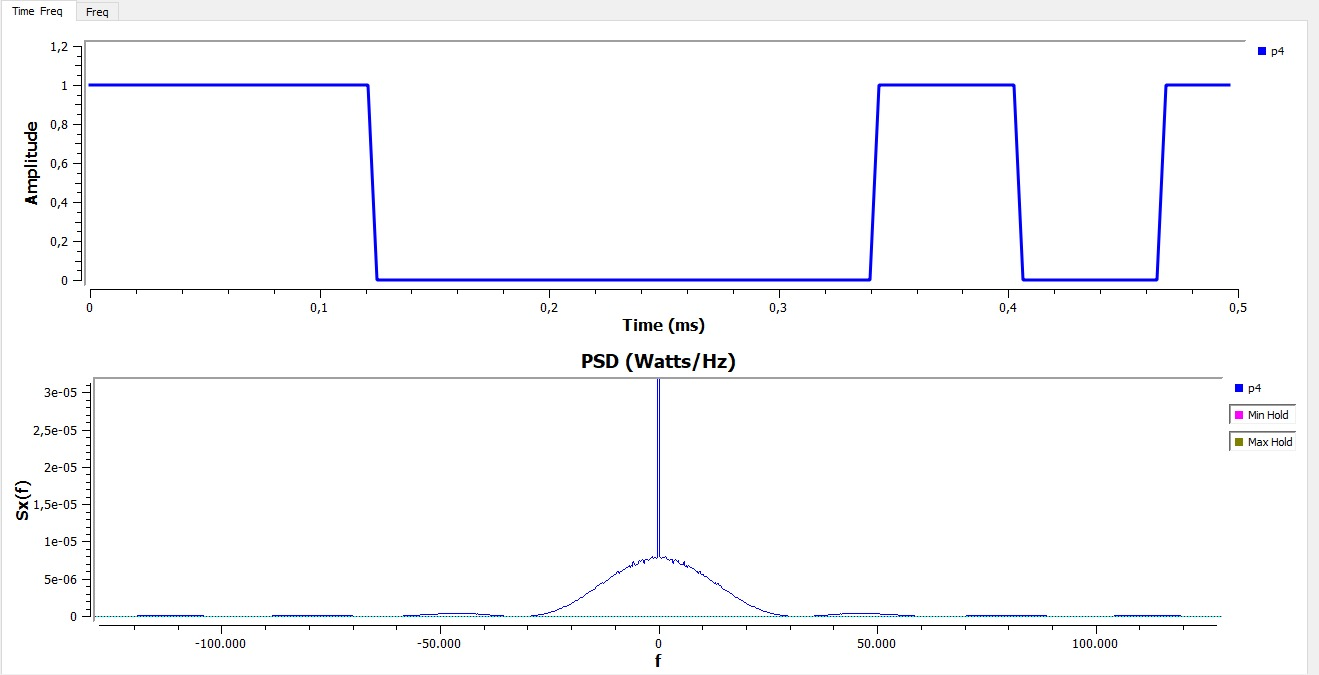
\includegraphics[width=0.6\columnwidth]{figs/psd_unipolar.jpeg}
    \caption{PSD of an unipolar NRZ signal}
    \label{fig:unipolar_PSD}
    \end{figure}

    \item In GNU you can also visualize the white noise, theoretically known to have a constant power over the entire frequency range, it is also a characteristic of the transmission signals and in the PSD you can see that noise with a constant power over a wide range of frequencies as shown in the Figure \ref{fig:figE}.

    \item Theoretically, the bandwidth of any digital signal or line encoding was infinite. However, various effects, such as the number of bits sent, could limit it. In general, the bit rate determined this behavior, as it was directly related to the bandwidth. Specifically, this was due to its dependence on frequency or sampling period. Additionally, this quantity was also based on the relationship between pulse width and the amount of information transmitted.

    \item The number of lobes that presented the PSD signal depended directly on the value of the \textit{SPS} variable, in the case of figure \ref{fig:figE} was performed with a value $SPS=6$, and it is observed that it has 2 lower lobes on each side, and the central one counts by 2, since it has twice the bandwidth.

    \item For the calculation of the frequency range occupied by the spectrum and if \textit{Sps} and \textit{Rb} are known, it is enough to make their product to obtain this range.

    \item The TDF computed N output points relative to previously sampled points within a time window, thereby defining resolution, equation shows us this relation: $f_{k} = \frac{f_{s}}{N}$

    For a more precise analysis of spectral lines, adjusting the number of FFT values would be necessary, typically increasing them to reduce resolution, albeit at the expense of increased computation time.

    \item When the value of the \textbf{K} parameter in the \textit{Unpack K Bits} block was modified, it means that the block had 16 bits to encode the input signal, in the case of audio, it can be seen in the figure \ref{fig:kbits} 16 peaks at different frequencies, which correspond to the harmonics of the signal, and the number of peaks increased because more precise harmonics could be found.
    \begin{figure}[H]
    \centering
        \centering
        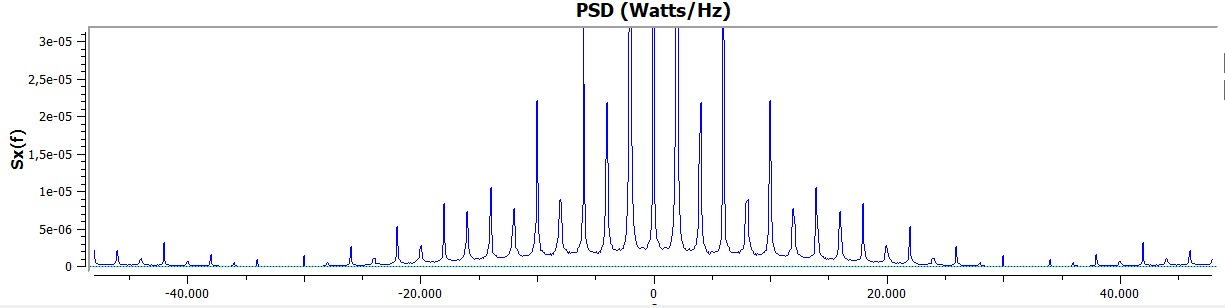
\includegraphics[width=0.9\columnwidth]{figs/K_bits.jpeg}
    \caption{Unpack K bits consequences}
    \label{fig:kbits}
    \end{figure}

    \item If the number of PSD lobes and the signal bandwidth are known, the sampling frequency can be calculated as: $f_{s} = N_{lobules} * R_{b}$

    \item The Unpack K Bits block reversed the packing process by separating K-bit packages into individual ones, typically resulting in a reduced output bit rate and sampling frequency, the following relation defines this result:     $fs_{out} = \frac{fs_{in}}{K}$.

    \item The Char to Float block did not affect the signal processing in the communication system, since it was only a data converter, so that the input bits could be processed.

    \item The case in which the PSD of a bipolar random binary signal is similar to the PSD of white noise, occurs when Sps=1 as shown in the Figure \ref{fig:FigC}, the PSD behaves very similar to that of white noise, this because the noise is much higher since the interpolator must enter many more samples, which contaminates the signal with noise and is similar to that of white noise.

    \item A vector was imposed to reflect the behavior of a straight line within the range [-1,1] in order to obtain the sawtooth wave. The parameter Sps remained at a multiplicative factor of 1, and a bipolar signal was utilized, as depicted in Figure \ref{fig:figTRANS}.    

    The resulting behavior demonstrated the utilization of a random bipolar signal, evidenced by phase shifts in certain components over time. Additionally, it was noted that disabling the random signal still allowed for achieving this behavior using the offset of the unipolar to bipolar conversion.

    \item In order to observe the unipolar RZ signal in the GNURadio scope like in figure \ref{fig:figTRANS}, some small changes had to be made in the flowchart:
    \begin{itemize}
    \item The variable h was manipulated in figure \ref{fig:figA}, so that the values 1 and 0 were repeated depending on the desired width, example: h = np.array([1,1,1,1,0,0,0,0]).
    \item The sum constant in the add block was eliminated to avoid negative values in the signal.
    \end{itemize}

    \item One change that can be made so that the random signal has Manchester NZR line encoding, is to modify the value of h so that it is ([1,1,-1,-1]). As shown in the figure \ref{fig:figTRANS}.
    
    \item Due to the fact that it was only possible to generate an OOK signal using a random unipolar signal, the program flow was modified to achieve this characteristic exclusively. The result of this modification was observed in Figure \ref{fig:figTRANS}.

    With this change, when the random signal was at 0, its state was defined as off. Additionally, the value of the Sps parameter was increased to improve interpolation and more precisely define the on and off states. This adjustment also resulted in an increase in the sampling frequency.

    \item The only change necessary to visualize the BPSK modulation in the flowchart was in the variable h, because in this variable we needed to define the sine function from $-4\pi$ to $4\pi$ with python functions. In addition, this modulation starts from a bipolar input, this is the reason why there is a phase change in the modulated signal, the change can be seen in figure \ref{fig:figTRANS}.

    \item To obtain a signal with ASK type coding, it is sufficient to change the values of the vector h in the form ([ 0.2,-0.5, 0.7, -1, 1 , -0.7,0.5,0.2]). As shown in the figure \ref{fig:figTRANS}.

    \item To generate the pulse signal, a vector was defined to follow the linear behavior of each peak of the signal, considering slopes of 0.1, 0.2, and even 0.3 in vector h. Additionally, the value of Sps was adjusted to achieve greater interpolation, allowing for better temporal definition of the signal. The input signal was left as a random bipolar signal, as observed in Figure \ref{fig:figTRANS}.

    \item The curly pulse function had complications, as it is the one that had the most changes in the flow chart. First, the input signal was defined as a bipolar, then the parameter h was designed to replicate the positive part of the function, i.e., a part of the increasing exponential, then a constant part, and finally a decreasing exponential, was defined in figure \ref{fig:W_h}. 

    In the interpolation block and together with the input bipolar signal, the output signal is reflected or designed depending on the input, but this is between negative and positive values, so it is necessary to put an offset at the output of the FIR, and thus keep the signal between 0 and 1. The entire flow chart can see in figure \ref{fig:W_flujograma}. 

    The result of the modulation can be seen in figure \ref{fig:figTRANS}.
    \begin{figure}[H]
    \centering

        \begin{subfigure}{0.9\columnwidth}
        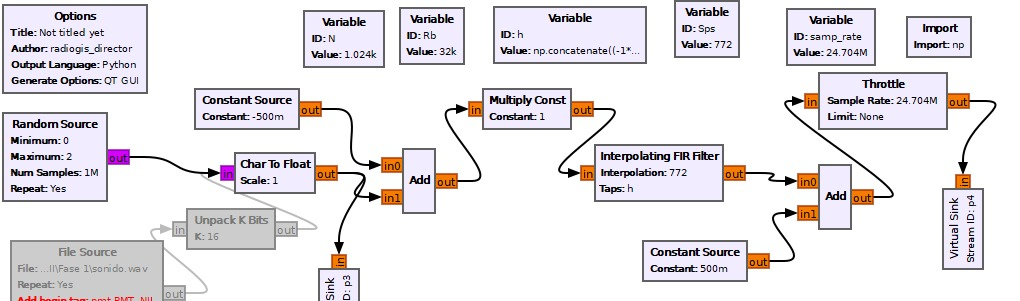
\includegraphics[width=0.7\columnwidth]{figs/pt_W_flujograma.jpeg}
        \caption{Flowchart of the rippled pulses}
        \label{fig:W_flujograma}
    \end{subfigure}
    
    \begin{subfigure}{0.9\columnwidth}
        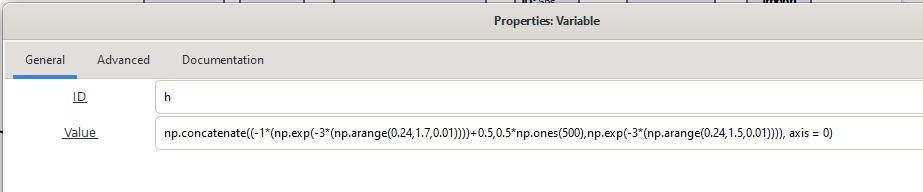
\includegraphics[width=0.9\columnwidth]{figs/pt_W_h.jpeg}
        \caption{Rippled pulses h variable configuration}
        \label{fig:W_h}
    \end{subfigure}
    \caption{Rippled Pulses}
    \end{figure}

    \item The difference observed in PSD of a bipolar signal and a unipolar signal is how the power is distributed in each. In theory a unipolar signal has a non-zero mean value \ref{fig:unipolar_PSD} (since it is never negative), which typically manifests itself as a peak in the PSD at zero frequency or DC. On the other hand, a bipolar signal \ref{fig:FigC} its power is distributed across the spectrum since it has a mean value of zero.
    
\end{enumerate}

\section{Summary}

\begin{enumerate}
 \item The PSD proved to be an important tool in this practice, providing a clear view of how the power of a signal was distributed across the frequency spectrum by providing a concise and powerful representation of how and where power was used in the transmitted signals we used. By analyzing PSD, we identified the presence of noise and other essential signal characteristics that affected the transmission of information. 

 \item Bipolar signals helped us in many of the signals proposed due to their ability to have their average value over time tends to be zero.
 This was beneficial because the absence of the continuum component meant a better PSD and the change of phase for the signals that needed that property.
 In contrast, a unipolar signal had its average value not in zero, which caused a DC level to show, however due to the requirement of some signals to not change their phase, it became helpful.

 \item Several tools were necessary to ensure the proper flow of data packets in the digital topology of GNU Radio. The sampling frequency, the number of samples per second, and the interpolation filter were critical for the accurate construction of the signals, as they determined how the data would be represented over time and frequency.

\end{enumerate}

% NO MODIFIQUE NI ELIMINE ESTA PARTE PARA QUE  APAREZCAN LAS REFERENCIAS
\bibliographystyle{IEEEtran}
\bibliography{bibliografia.bib}\nocite{*}

\end{multicols}
\end{document}